\documentclass{webofc}
\usepackage[varg]{txfonts}   % Web of Conferences font
% 
% Put here some packages required or/and some personnal commands
%
%
\begin{document}
%
\title{EsbRootView, a portable event display for the ESSnuSB project}

\author{
  \firstname{Guy}
  \lastname{Barrand}
  \inst{1}
  \fnsep
  \thanks{\email{barrand@lal.in2p3.fr}}
  \fnsep
  \footnote{On behalf of the ESSnuSB project.}
}

\institute{
  Laboratoire Ir\`{e}ne Joliot-Curie, Universit\'{e} Paris-Sud, CNRS-IN2P3, Orsay, France
}

\abstract{%
  EsbRootView is an event display for the detectors of ESSnuSB able to
  exploit natively all the nice devices that we have in hands today;
  desktop, laptops, but also smartphones and tablets.
}
%
\maketitle
%
\section{Introduction}
\label{intro}
The goal of the ESSnuSB project \cite{ESSnuSB} is to discover and measure neutrino
charge-parity violation with unprecedented sensitivity. The ESSnuSB
concept takes advantage of two outstanding opportunities. The first is the construction in Europe of the European Spallation
Source, ESS, the world’s most intense proton source, with a beam power
almost one order of magnitude higher than any other accelerator. The
second is the measured unexpectedly large value of the
oscillation mixing angle $\theta_{13}$. The latter fact implies that to obtain maximum sensitivity, the neutrino detector shall be placed at the second neutrino oscillation maximum, not at the first as implemented by other proposed experiments. The Garpenberg mine in Sweden, in which it is proposed to install the underground neutrino detector, is situated at a distance from ESS that corresponds to the second maximum.
The goal of the ESSnuSB H2020 Design Study is to organise European physicists and accelerator engineers in co-operation with the ESS Laboratory and the Garpenberg Mining Company to study and produce a Conceptual Design Report for the ESSnuSB project.

In the work package five of the ESSnuSB project we developed an event display based
on the graphics technology developed at Orsay from 2010 (developments
done at LAL up to 2020 and now continued in the new Orsay IN2P3 IJCLab
laboratory that absorbed LAL).
This technology permits to have programs
running natively on most of today's interactive devices as desktop/laptop under
Linux, macOS or Windows-10 but also on iOS/Android smartphones and
tablets. Since 2019, with the same core technology we can run in most
web browsers by using the WebAssembly and WebGL technologies.

Today's versions 3.x can visualise simulations data of the ``neard'',
``fard'' and ``fgd'' detectors. The small neard is intended to monitor the
beam of neutrinos and the fard is the big Cherenkov one
placed at the second neutrino oscillation maximum. The fgd is a detector
composed of a 3D array of scintillator cubes, which can be read out
semi-independently, and placed in front of the neard.
The ESSnuSB setup
is nicely explained in the ``ESSnuSB Design Study Project'' video that
could be found on YouTube or through the main web page of the project
at https://essnusb.eu.

\section{Main ideas}
EsbRootView is fully written in C++ (98 flavour) with good part of the code being
pure header. Being able to run on most interactive devices, including
iOS and Android, is made possible by the fact that since C++98 and GL-ES (OpenGL for Embedded
Systems, a graphics rendering standard), are available for all of them.
A key point is that at Orsay we have light portable code (inlib/rroot
classes) to read ROOT files and then we can read on all our devices the files describing the detectors and
the events issued from the ESSnuSB detector simulations.

We have implemented an event model with a one\_event class managing
instances of EsbMCTrack, EsbDetectorPoint, EsbHit, EsbFgdHit classes
describing data issued from the simulation. All the items of the event
model received one or more graphical representations. For the geometries, we can read the TGeo classes stored in the ROOT
files and we have graphical representations of them in our inlib
library. To view geometries, we have nothing specific to ESSnuSB.

To let the user customise things, we have a default Bourne shell like scripting, the
``insh'', which is described below in section \ref{insh}.

About our event model, we are aware that this duplicates
the event model code found in the EsbRoot framework used for the
simulation, but for the moment this one is not portable, in particular
because it is tied
to CERN-ROOT \cite{CERN-ROOT}, and then not usable for us. Being able
to have a portable unique event model shared with the simulation and analysis would be a
nice target to aim for the mid and long range term of the ESSnuSB project.

\section{inlib/sg}
The core of our graphics technology is the usage of a scene graph
logic developed at Orsay; the inlib/sg classes (sg for scene graph).
inlib/sg is strongly inspired of the great OpenInventor developed by
Silicon Graphics Incs in the 1980's \cite{OpenInventor}. The idea is to describe a scene
by using a graph of nodes. A node could be an instance of a camera
class (inlib::sg::ortho, perspective) specifying the position, orientation and depth of view of a
camera, an instance of a 4D matrix class (inlib::sg::matrix) to position an object in a 3D
space (rotation and translation) or an instance of a shape node
describing for example a cube (inlib::sg::cube). A key node is a group
(inlib::sg::group) to gather nodes.

Whence having built a scene graph, the rendering is done, typically
after having received some expose event in a drawing area window, by
applying a ``render\_action'' that traverses the scene graph and asks to the
nodes the actions that will be passed to a specific graphics engine.
For example a shape node (cube, sphere, polyhedron), when traversed,
will give to the render\_action the graphics primitives (points, lines, segments, triangles)
representing that shape. A camera node will give a
projection matrix, a matrix node will give a model matrix. A common graphics engine
being GL-ES, we have the exlib::sg::GL\_action
class that does that for GL-ES. But we have also various render\_action
to do offscreen rendering, web rendering (using WebGL) or to handle private
company specific engine, such as the Apple/Metal one.

Note that we keep within the namespace ``inlib'' only code that relies
on the STD/STL and on some few system functions not being in C++98.

\section{exlib}
The code that depends on external libraries, as GL-ES, is within the
exlib namespace. A typical example is the GL-ES related code in
exlib::sg::GL\_action, or the code that handles various ``windowing''
technologies, for
example the exlib::X11::viewer and exlib::Windows::viewer classes for
X11 or Windows. By
windowing we mean the code to create a window to draw in and get events
as click or touch on it. Note that the
exlib::sg::GL\_action inherits the virtual inlib::sg::render\_action
which is the only one seen by the inlib::sg nodes. The relation of the rendering
toward the scene graph nodes is abstracted.

\section{Graphical User Interface}
In EsbRootView the GUI is done with inlib/sg scene graphs.
This permits to have the same look and feel on all platforms.
For the moment we follow the logic of video games,
mainly we give high priority to the ``scene'' which takes the full
window (then full screen on smartphones and tablets), and we pass in ``GUI
mode'' when needed by clicking/touching the bottom area of the window.
The GUI mode leads to a central menu list with, for example, the
``setup'' menu items permitting to choose which detector to work with
(neard, fard, fgd). Central menu items may lead to sub menus. A bottom-left ``home'' button permits to return to the top
menu list. A bottom-right ``back'' button permits to return one level
back
in the central menu tree. A left ``params'' button permits to setup global
parameters. And at last, a ``camera'' button on the right permits to return
also to the ``scene mode'' but by mapping tiles of squared buttons at
left and right of the window to do various common actions; the right
tiles are dedicated to camera settings and the left ones to common
actions as doing a ``next event'', clearing the scene, do a ``view
all'', switching on/off the light, producing a jpeg or png, etc...
When in scene mode, a ``background popup'' leads 
to a shortcut to various global actions, and if in ``picking mode''
(setup from a tile button on the right), a contextual popup appears when
picking an object in the scene. Contextual menu items permit for
example
to center the camera on the picked object, get infos about it, change its colour, etc...

 Our GUI is perhaps not the most beautiful and sophisticated, but it is functional and works the
 same on all platforms. Due to the fact that it is based on the same
 graphics technology as the scenes, it does not have to involve
 an extra third party package, which simplifies a lot the building
 of the application and its distribution.

\section{scripting with insh}
\label{insh}
 EsbRootView is equipped with the core of a Bourne like shell called
 "insh" for INlib SHell. It had been introduced to have a way to
 customise things by using a scripting syntax known by any UNIX
 pedestrian and easily implementable by a "doer" in a light way. insh has the basic
 mechanisms found on any bash shell: variables, env variables, dollar
 replacement of a variable, backquoting, execute other scripts, source other
 scripts and, obviously, execute commands with options. For example, in
 a ``next event'' insh script, you may see:
\begin{verbatim}
    # this is a comment.
    event_index=`event_index`
    gui_show_console ${event_index}
    scene_clear_dynamic
    event_vis MCTrack -color=red
    event_vis WCDetectorPoint -color=green
\end{verbatim}
 
\subsection{Terminal mode}
On desktop versions (macOS, Linux, Windows), the program can be
started with the "-terminal" option that permits to type insh commands
from the terminal. The behaviour is similar to the bash prompt.
In particular by typing twice the tab key you activate the completion and have the list of available commands.
For all commands, the user has a help text that can be read by using the help command:
\begin{verbatim}
    EsbRootView> help echo
    EsbRootView> help event_model
\end{verbatim}
Around two hundred commands exist now in EsbRootView. The reference manual
of all of them can be found in the web pages (see section \ref{web_pages}).

The terminal prompt handles a history maintained under the user
Documents/EsbRootView/.insh\_history file. The history logic is the
same as for a bash prompt; type "history" to see the numbered past
commands, ``exclamation mark and number'' to recall a numbered command,
and twice exclamation mark to execute again the last command.

 \subsection{The startup, event, anim.insh scripts}
 The ``setup'' main menu item permits to choose which detector to work
 with. Depending on the selection, dedicated startup.insh, event.insh, anim.insh
 scripts are copied from internal versions coming with the
 installation (from the ``resources'' directory) into
 the user Documents/EsbRootView directory. The startup.insh script is
 executed at each startup of EsbRootView, the event.insh when doing a
 ``next event'' and the anim.insh when applying the ``scene anims''
 main menu item. These scripts are good starting points to customise
 the general overall behaviour of EsbRootView. 

\subsection{event\_model, event\_next, event\_vis: the commands to know}
  The event\_model command lists the event model classes (MCTrack,
  WCDetectorPoint, FgdDetectorPoint, FgdHit from 2.x versions) along
 their fields (for example MCTrack pdg, x, y, z, p, E, etc...). The event\_next  permits to have an event taken from the
 current opened event file. The event\_vis permits to visualise an item of the event model
 instances in the current loaded event. Its first argument is the wanted item
 and other arguments are ``-options''. For example:
\begin{verbatim}
    event_vis <event_model_class> [options]

    event_vis MCTrack -cut=(pdg==50000050) -color=red

    event_vis WCDetectorPoint-cut=pdg==50000050 -color=red
    event_vis WCDetectorPoint -cut=pdg!=50000050 -color=blue -point_size=4
\end{verbatim}
  The -cut logic, as described below in \ref{cut}, applies also for the event\_count, event\_stats and event\_print commands:
\begin{verbatim}
    event_print <event_model_class> [options] [fields]

    event_print MCTrack -cut=(pdg==50000050)
    event_print MCTrack -cut=(pdg==50000050) x y z p

    event_count MCTrack -cut=(pdg==50000050)

    event_stats MCTrack -cut=(pdg==50000050) p t
\end{verbatim}
  As explained in "help event\_stats", event\_stats prints the
  sum/min/max/mean/rms for the fields of the selected/cut objects.

\subsection{The -cut option}
\label{cut}  
  A useful option found on all
  ``event\_'' commands  is the ``-cut'' option that permits to filter
  instances of an event model item according to their field
  values. This option is implemented with a little interpreter (done
  with lex and yacc) that has the syntax of  a C conditional statement.
  For example, in an insh script, it permits to do:
\begin{verbatim}
    cut_first="(pdg==50000050)&&(is_secondary==true)"
    cut_second="(pdg==50000050)&&(is_secondary==false)"
    ...
    event_vis MCTrack -cut=${cut_first} -color=red
    event_vis MCTrack -cut=${cut_second} -color=green
    ...
    event_vis WCDetectorPoint -cut='x>0' -color=blue
\end{verbatim}
  
\subsection{The -modeling option}
\label{cut}  
  We can have multiple representations for an event model item. For
  example, the MCTrack has the ``point' (default), ``arrow'' and
  ``markers'' ones. (``arrow'' draws an arrow at MCTrack position in
  the direction of its momentum).
  By playing with the -cut and  -modeling options, someone can view the topology of a muon decay as
  in figure~\ref{fig-muon-decay}.

\subsection{The pdg and particle\_print commands}
 Among commands, must be mentioned the pdg and particle\_print ones
 that permit to dump tabular informations about particles. Type ``help pdg'' or ``help
 particle\_print'' for more.

\section{Plotting. event\_histo, event\_plot commands}
  Making histograms and filling ntuple are basic tools in HEP. Plotting
  used to visualise histograms (and ntuple ``projections'') is an
  important tool in HEP for doing analysis. The inlib/sg library comes with
  the inlib::sg::plotter node that permits to visualise
  histograms done with the inlib::histo::h1d, h2d
  classes. The plotting is then done with
  the same scene graph logic as for visualising detectors, events
  and making the GUI: in EsbRootView we have a unified graphics.
  See figure~\ref{fig-layout-event-1} and figure~\ref{fig-fard-setup} for
  examples.

   EsbRootView permits to create histograms from items in the event
  model and plots them in scene mode by using the event\_histo and
  event\_plot commands. For example:
\begin{verbatim}
    event_histo MCTrack -name=h_MCTrack -cut=(pdg!=50000050) -xfill=p
    event_plot MCTrack -cut=(pdg!=50000050) -xfill=p
\end{verbatim}
  Type ``help event\_histo'' or ``help event\_plot"' for more.
  
\section{Animations}
 EsbRootView comes with a nice mechanism to do animations. The 3.x
 versions come with animations showing the tracking of optical photons
 coming from the Cherenkov effect of charged particles in water. It permits to see the ``smoke rings' of
 a muon and how photomultipliers switch on when receiving light. It reinforces the
 intuition about how things happen when, for example, a
 muon decays in the neard or fard detector.
 These rings could be seen in the YouTube video ``ESSnuSB Design Study
 Project'' both for the neard and in the fard. See
 figure~\ref{fig-youtube-neard}, figure~\ref{fig-youtube-fard}. 
 
\section{Platforms}
In general, we arrange to use the default solutions provided by the
device providers for the windowing, the rendering and the
compiler. This permits to get the best performances on each kind of
device and also simplifies the build by not having to install too
many third party packages.

\subsection{Linux}
On Linux, we use X11 for the windowing, the Mesa OpenGL for the
rendering and the g++ compiler. The build is done by using our
``bush'' set of bash scripts. (Bush is for BUild with (Bourne) SHell).

\subsection{macOS}
On macOS, we use Cocoa for the windowing, the Apple OpenGL for the
rendering and the clang++ compiler coming with Xcode. Since at the 2018 WWDC
conference Apple deprecated its OpenGL in favour of its Apple/Metal
rendering layer, in 2020, we did a first version of a
exlib::metal::action to switch to Apple/Metal when needed. We have a
first version of EsbRootView that works on Metal, but it is not yet
fully implemented and optimised. Therefore, we prefer to deliver with
Apple/OpenGL as long as it is still available.

\subsection{Windows}
On Windows, we use the standard WIN32 API for the windowing, the
Microsoft opengl32.lib for the rendering and VisualC++ for the
compiler (the cl.exe command). VisualC++ can be installed and used
with a free version of VisualStudio brought from Microsoft web sites.
The build is done under CYGWIN by using our ``bush'' set of
bash scripts. The usage of the VisualC++ from here is done by using a ``bush/vc++'' script
encapsulating the usage of the cl.exe command in a way that the
arguments passed to bush/vc++ have the same syntax than for a g++ command.

Note that today we do not use DirectX for the rendering, but our
architecture would permit to have a straight
exlib::Windows::DirectX\_action class for
the rendering if one day or another Microsoft would deprecate its
OpenGL implementation.

\subsection{iOS}
On iOS we use the UIKit for the windowing, the Apple GL-ES for the
rendering and the clang++ compiler coming with Xcode. We have not yet
an Apple/Metal version for the rendering. It is in the job list, but in
principle the exlib::metal::action done for macOS should be reusable
``as is'' for iOS.

Note that here we use Xcode on a Mac to build the application. Xcode is more or
less mandatory if wanting to deliver for the iOS App Store or upload,
in a simple way, the cross compiled application on an iPhone or iPad.

Today EsbRootView had not been deposited on the macOS and
iOS App Stores, but it is in the job list to do so.

\subsection{Android}
To build for Android, we use the SDK and NDK developments kits to
cross compile the application from a Mac. We use some minimal java for the windowing (to create an ``activity'')
but use the C EGL library of the NDK for the rendering. We build the
``EsbRootView.apk'' by using the SDK tools (ant and GNUmake) along the
adb program to upload the apk on a device connected to the Mac.

Today EsbRootView had not been deposited yet on the Google
Play Store, but it is in the job list to do so.

\subsection{WebAssembly}
 For visualisation in the WWW, we use WebAssembly \cite{WebAssembly}. In most web browsers there
 is a virtual machine (the wasm) that permits to execute a C++
 application locally. By installing the emscripten SDK on a Mac or a Linux, someone can cross compile
 (with the emc++ compiler) a C++ application to produce a wasm binary. The windowing is done by using a
 ``canvas'' of the web browser, and the rendering is done by using WebGL.
We did a exlib::wasm::render class that produces, then from the C++ in
the wasm binary, a textual javascript code to order the rendering of
primitives in the web browser by using WebGL. The SDK provides an
index.html file along some javascript files to create the WebGL
canvas, download and activate the wasm binary.

The overall build is done again with our ``bush''  set of bash scripts. At the end we have the wasm
binary, several html and javascript files that can be deposited in
static web pages. There is no need to have dedicated web servers to
deliver this web application. There is a WebAssembly version of
EsbRootView accessible from the EsbRootView section of the ``softinex
portale'' under the gbarrand.github.io web pages. (``softinex''
\cite{chep13-tools} is the
entity that gather all our applications done with our inlib and exlib libraries).

After having passed the startup, that needs to
download and activate the wasm binary, the user experience is rather
good. Anyway the overall reactivity of the web app is not so good than the native
application. This is due to the fact that here we are pilling up
layers as running
inside a virtual machine, doing ``javascript string programming'' to do the
WebGL and then having the WebGL activating the native GL-ES from javascript.
All these layers induce
inefficiencies compared to a native version. This being said the fact
to be able to deploy world wide so easily is definitely great.

Today the overall EsbRootView application probably asks too much at
the level of the graphics to have a nice and fluid user experience with
the web version. For the web, one idea would be to have a more light version dedicated
for outreach.

\section{Web pages and repositories}
\label{web_pages}
The web pages of EsbRootView are at https://gbarrand.github.io under
the section ``EsbRootView'' at left.
The source code of stable releases is on github at
https://github.com/gbarrand/EsbRootView.git. The license is a
customisation of the FreeType license. For each release, we
arrange to provide binaries at least for Linux, macOS and Windows.
A WebAssembly version is available through the web pages.

\section{Geant4/g4tools}
Must be mentioned that our inlib/exlib classes are not so foreign to
HEP since it is delivered under the namespace ``tools'' in Geant4 \cite{geant4} as a
baselayer to the analysis ``category'' to do the histograms,
ntuples, IO at various formats (ROOT, csv, HDF5) and offscreen plotting
with our scene graph logic. See \cite{chep13-analysis} and \cite{chep16-analysis} .

\section{Conclusions}
EsbRootView is probably the first HEP event display written in C++ able to exploit
natively all the nice devices that we have in our hands today, including
desktops, laptops but also smartphones and tablets. Its flexible
architecture permits also to have a web version done on the same C++
core as for the other platforms. It permits to have
animations that strengthen the intuition about what happens in the
detectors. Its scripting mechanism, inspired by the Bourne
shell permits a strong customisation with a short learning curve.

Up until now, EsbRootView proceeds well. The only downside that we see is
the inability to have common event and detector models, along a
coworking IO service, shared with the other parts of the ESSnuSB software.
The lack of portability of the IO service and of frameworks in general is a quite common
problem in HEP that, we think, refrains this field to enjoy fully
all aspects of computing technologies that we have today. ESSnuSB being a long
term initiative, if fully considering interactive technologies now, could show the
way on these points.

\section{Acknowledgments}
This work was supported by the COST Action CA15139 EuroNuNet and by the European Union research and innovation programme Horizon 2020 under the project ESSnuSB (Grant Agreement No 777419).

\begin{thebibliography}{}

\bibitem{ESSnuSB}
  M. Dracos, E. Baussan, E. Bouquerel, T. Ekelof, A. Kayis Topaksu,
  ``The ESSnuSB Project'',
  Proceedings of Science. The 21st international workshop on neutrinos
  from accelerators (NuFact2019) \textbf{369} (2020).
  
\bibitem{CERN-ROOT}
 R.~Brun and F.~Rademakers,
 ``ROOT - An Object Oriented Data Analysis Framework'',
 Nucl. Inst. Meth. in Phys. Res. \textbf{A 389}, 81 (1997).

\bibitem{OpenInventor}
  Josie Wernecke,
  \textit{The Inventor Mentor}
  (Addison-Wesley, 1994)

\bibitem{WebAssembly}
  A.Haas, A.Rossberg,  D.L.Schuff,  B.L.Titzer,  M.Holman, D.Gohman, L.Wagner, A.Zakai, JF.Bastien,
  ``Bringing the web up to speed with WebAssembly'',
  Proceedings of the 38th ACM SIGPLAN Conference on Programming
  Language Design and Implementation 185–200 (2017)
  
\bibitem{chep13-tools}
  Barrand G,
  ``softinex, inlib, exlib, ourex, ioda, g4view, g4exa, wall'',
  J. Phys.: Conf. Ser. \textbf{513}, 022002 (2014)

\bibitem{geant4}
  Agostinelli S et al,
  ``Geant4—a simulation toolkit'',
  Nucl. Instrum, and Methods \textbf{A506}, 250-303 (2003)

\bibitem{chep13-analysis}
  Hrivnacova I,
  ``Extending Geant4 Parallelism with External Libraries (MPI,TBB) and Its Use on HPC Resources'',
  J. Phys.: Conf. Ser. \textbf{513}, 022014 (2014)

\bibitem{chep16-analysis}
  Hrivnacova I, Barrand G,
  ``Analysis Tools in Geant4 10.2 and 10.3'',
  J. Phys.: Conf. Ser. \textbf{898}, 042018 (2017)

\end{thebibliography}

\begin{figure}[ht]
\centering
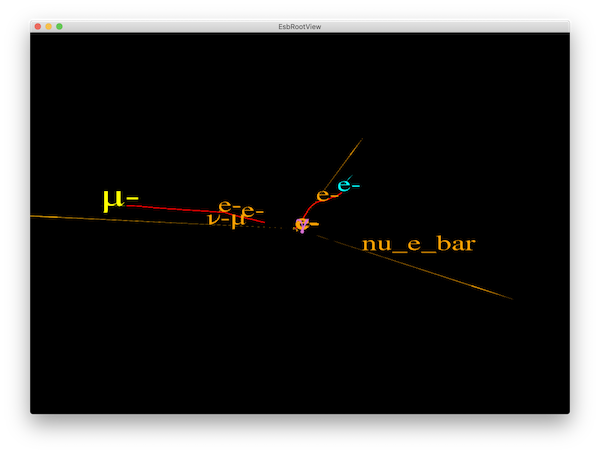
\includegraphics[width=10cm,clip]{neard_MCTrack_arrow}
\caption{A muon decay topology.}
\label{fig-muon-decay}
\end{figure}

\begin{figure}[ht]
\centering
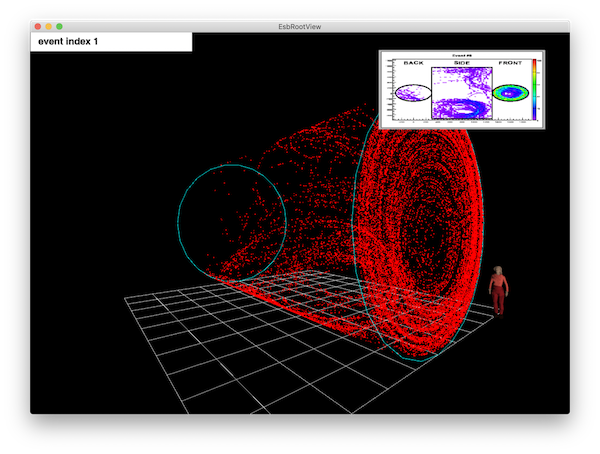
\includegraphics[width=10cm,clip]{layout_event_1}
\caption{DetectorPoint instances in the neard.}
\label{fig-layout-event-1}
\end{figure}

\begin{figure}[ht]
\centering
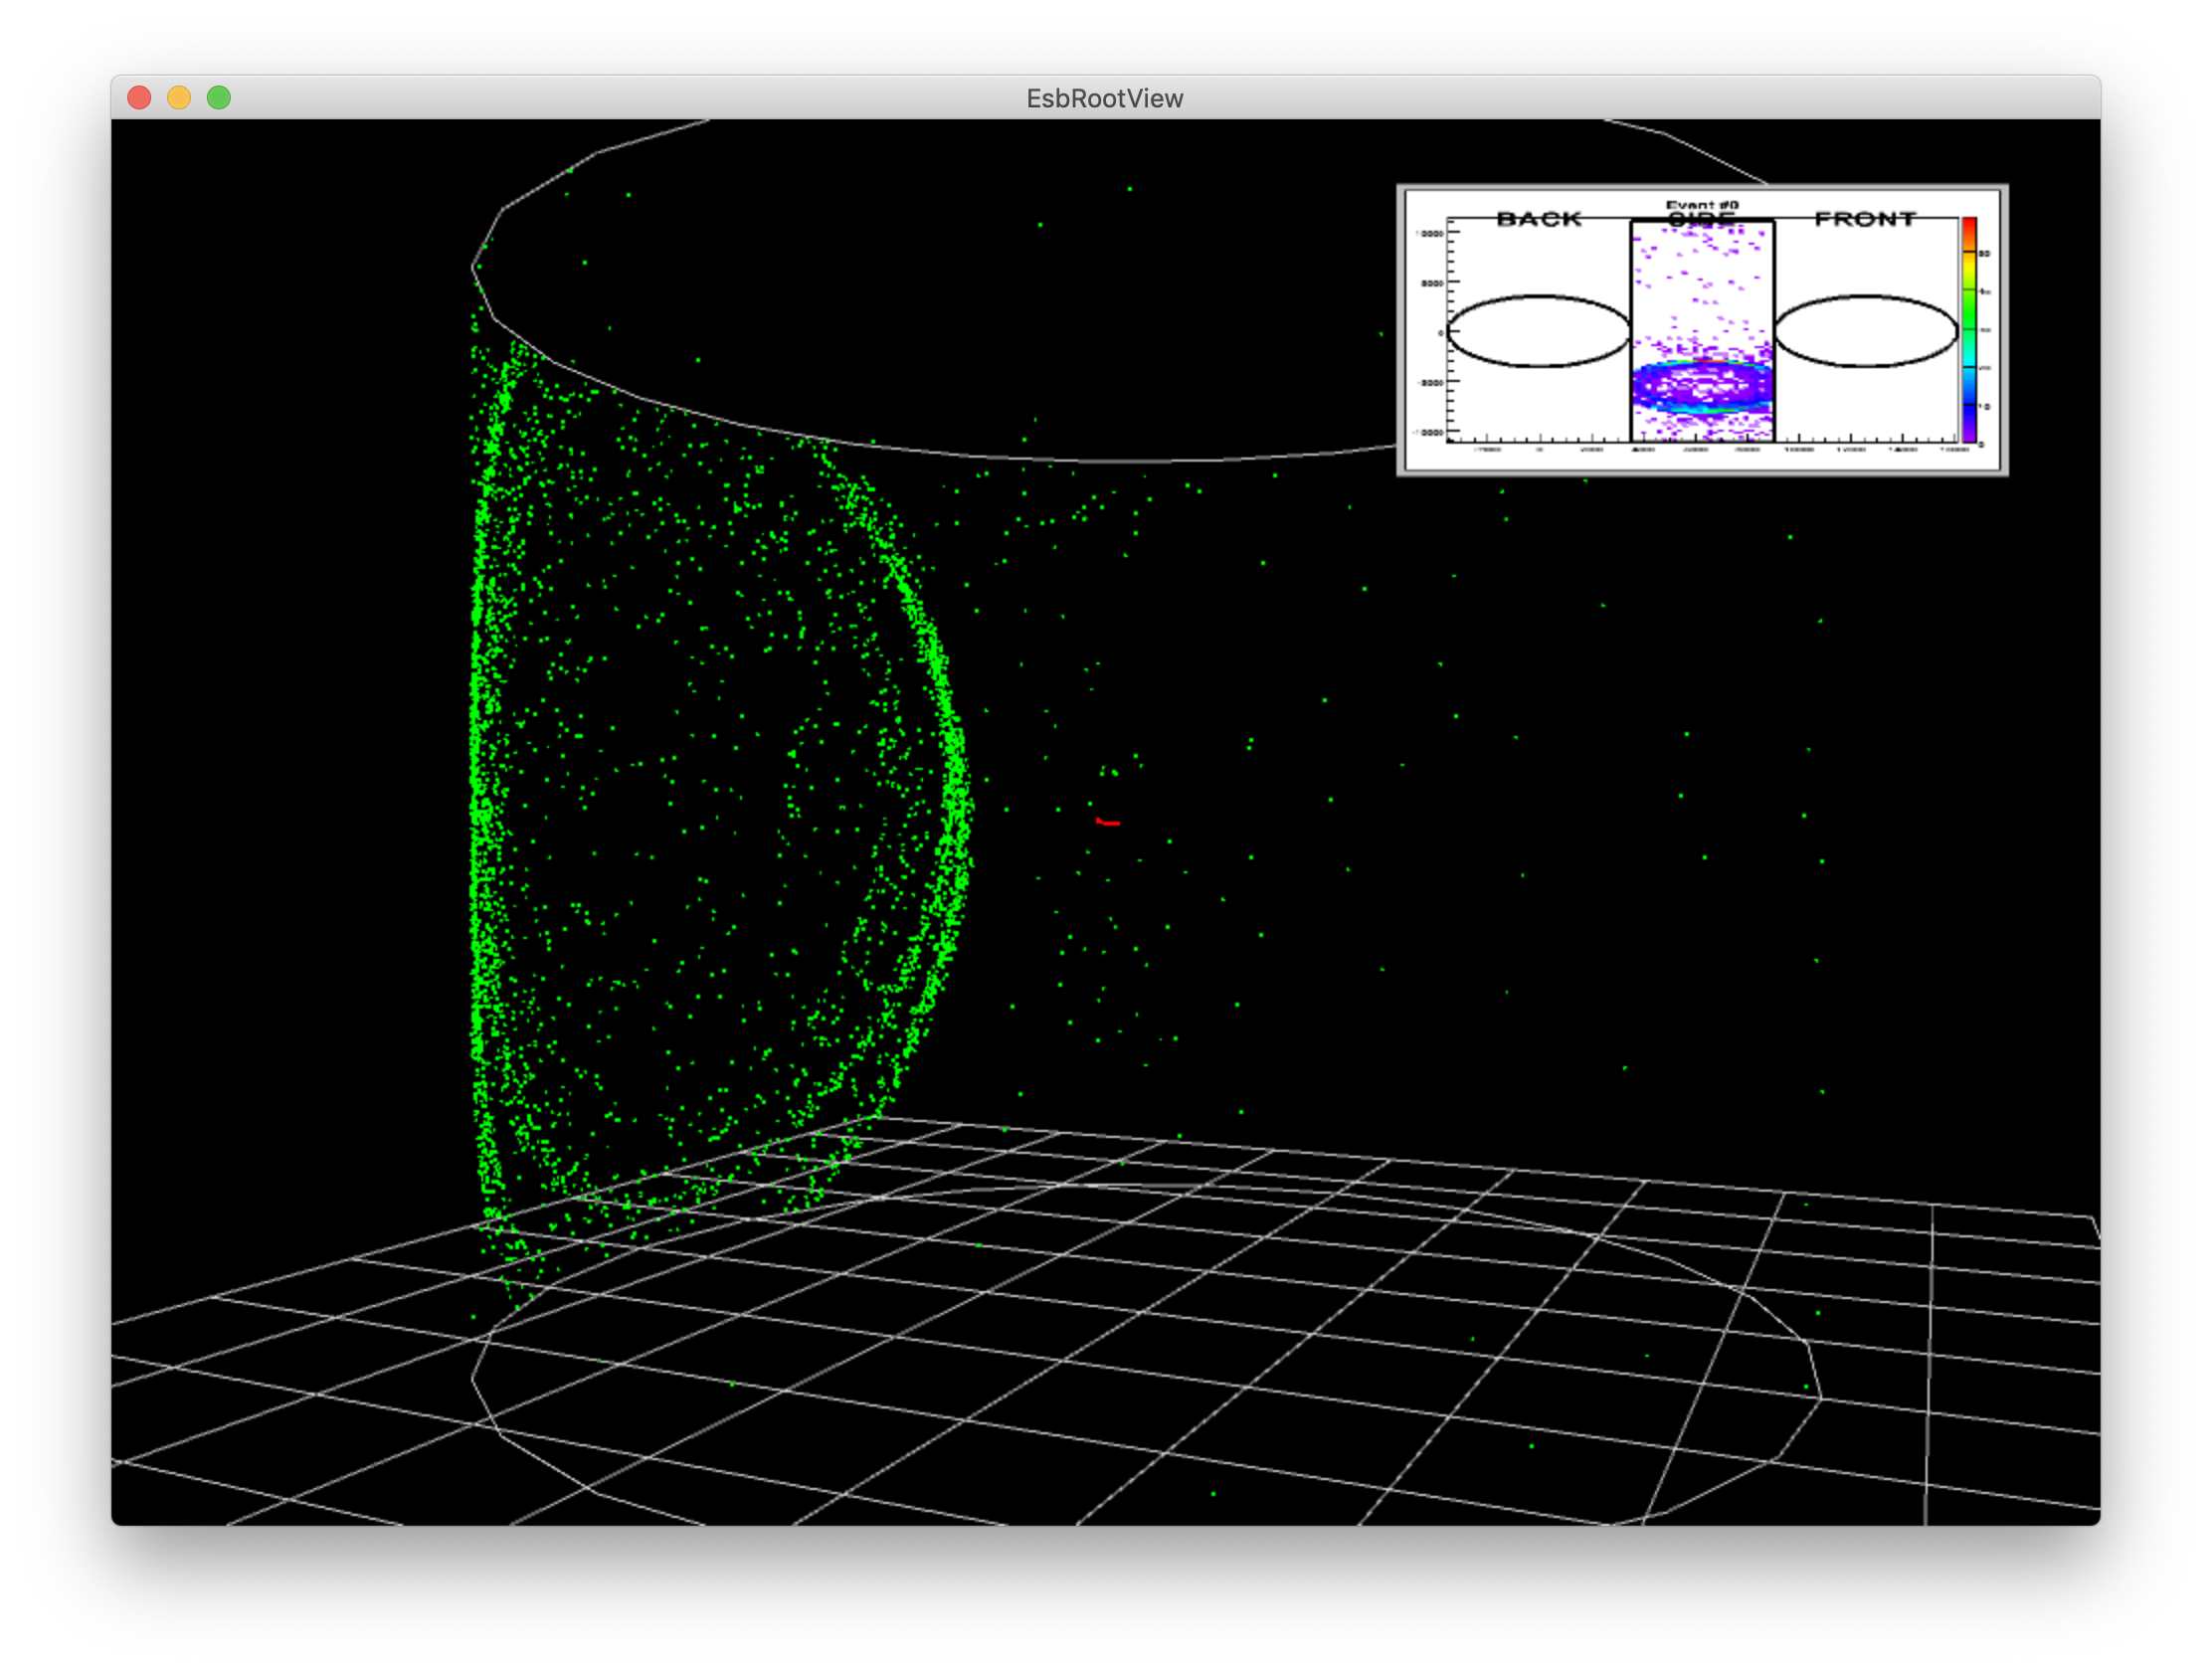
\includegraphics[width=10cm,clip]{fard_setup}
\caption{DetectorPoint instances in the fard.}
\label{fig-fard-setup}
\end{figure}

\begin{figure}[ht]
    \centering
    \begin{minipage}{0.45\textwidth}
        \centering
        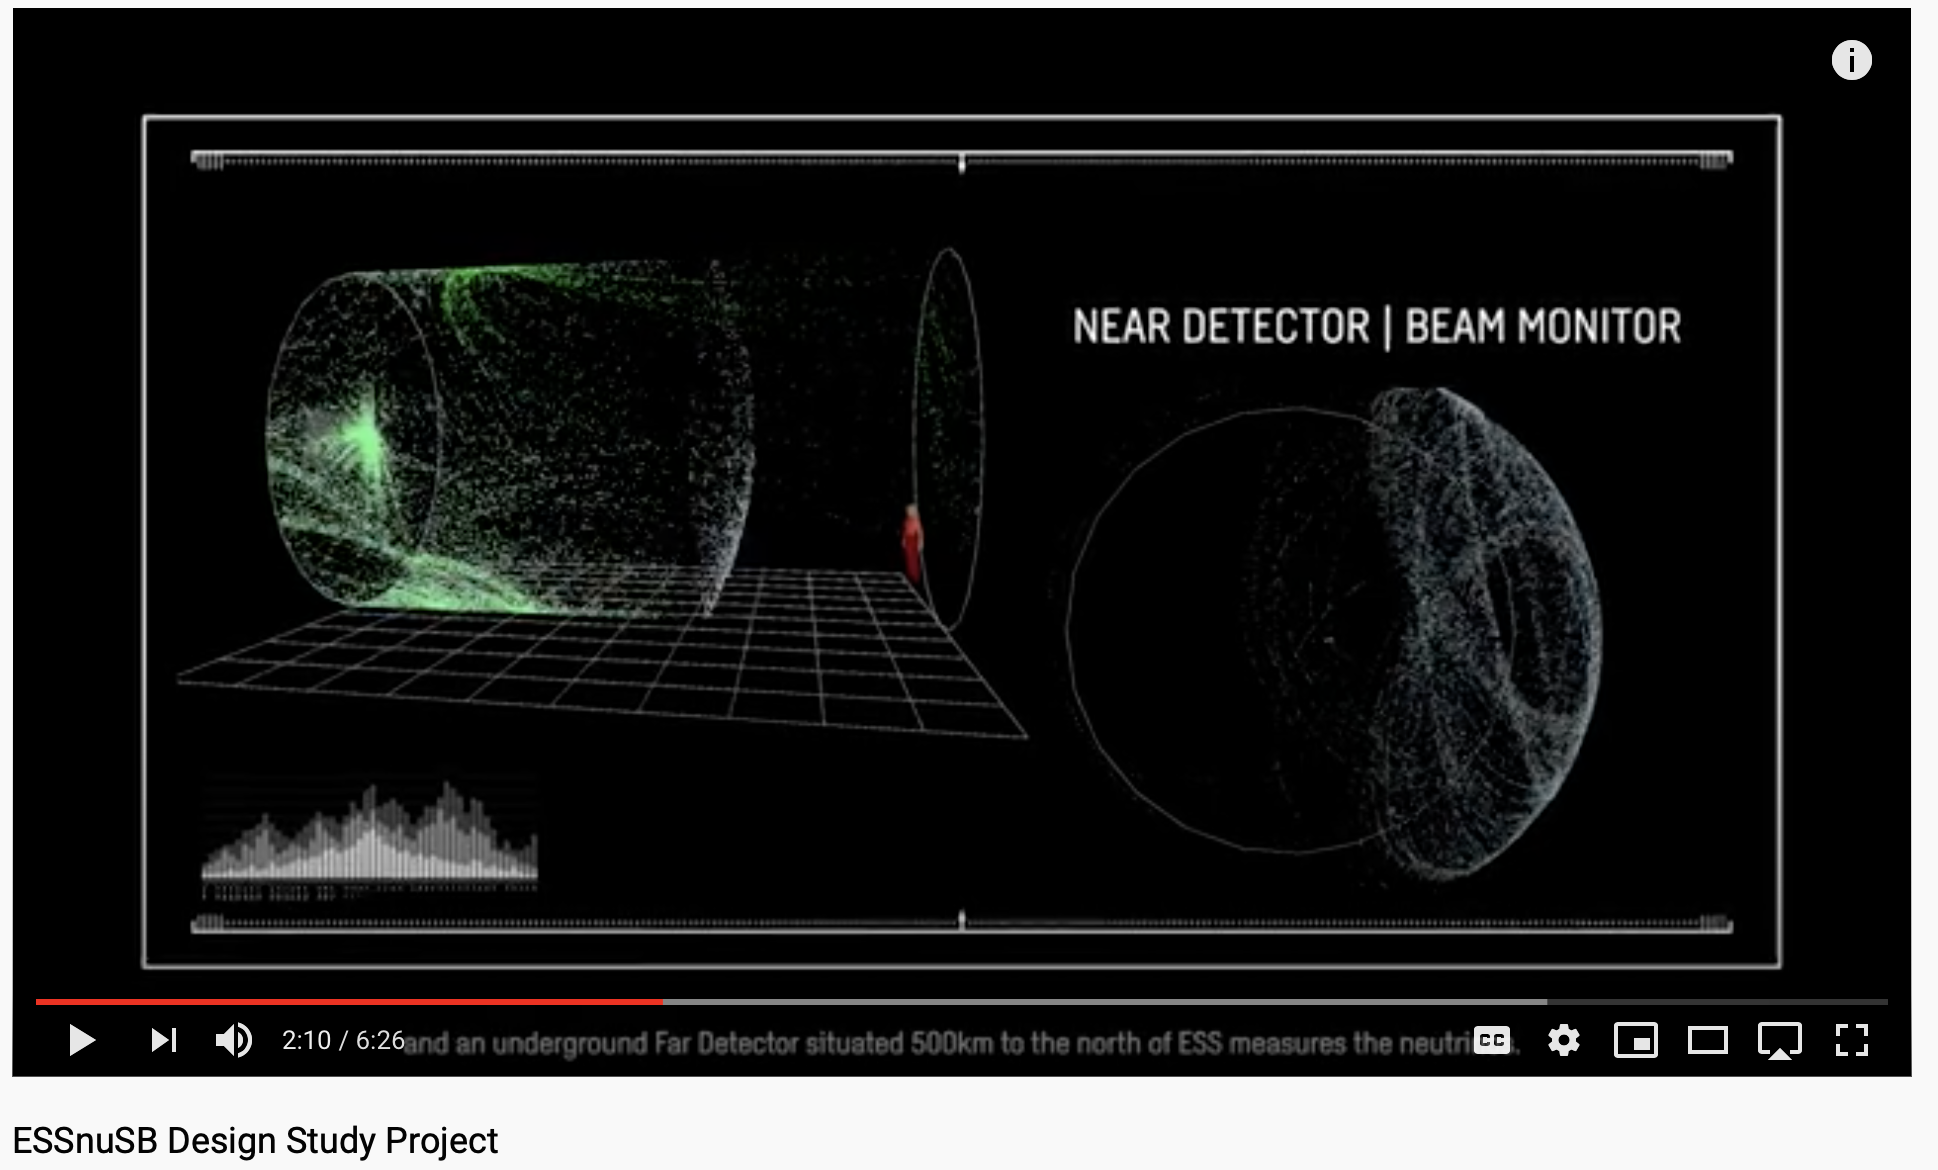
\includegraphics[width=7cm,clip]{youtube_neard}
        \caption{Cherenkov light deployment in the neard}
        \label{fig-youtube-neard}
    \end{minipage}\hfill
    \begin{minipage}{0.45\textwidth}
        \centering
        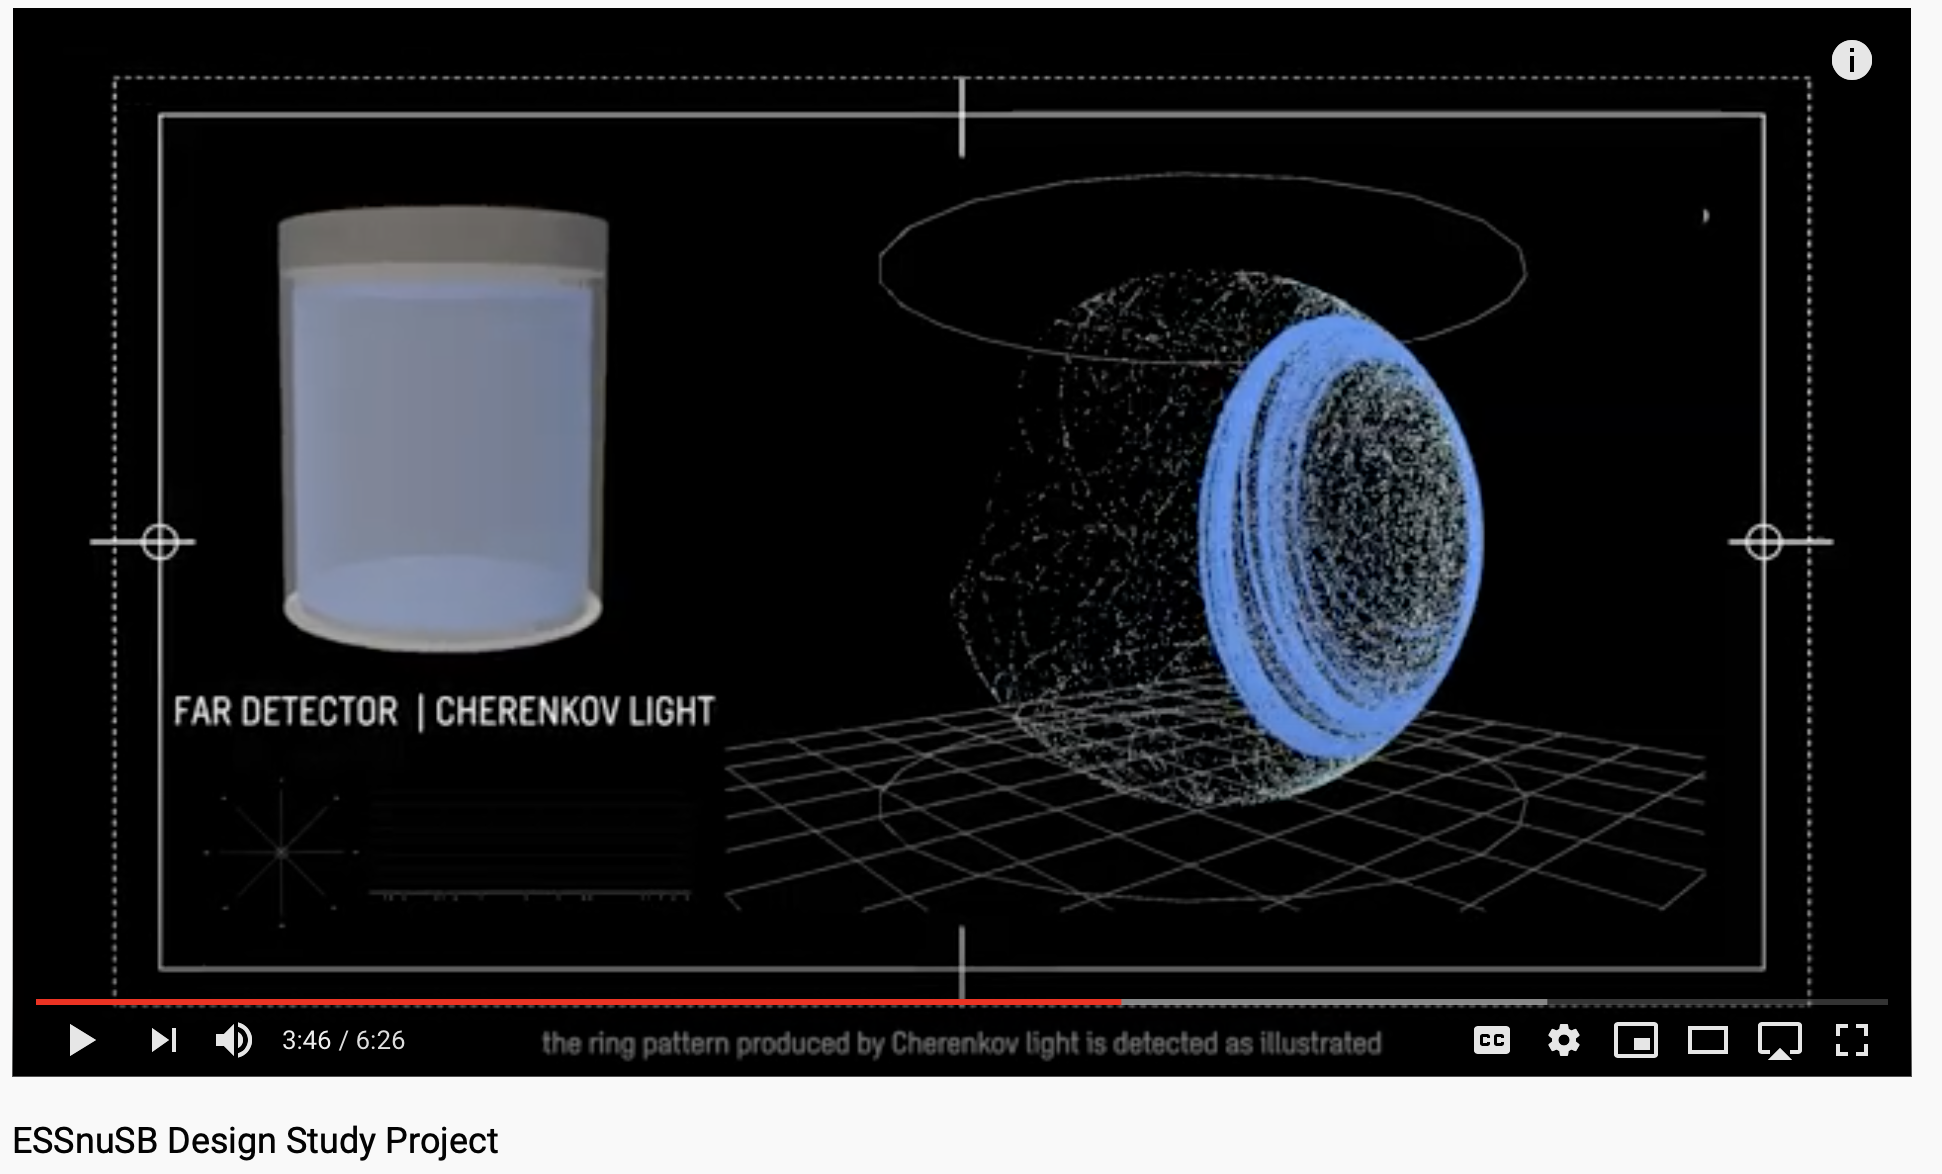
\includegraphics[width=7cm,clip]{youtube_fard}
        \caption{Cherenkov light deployment in the fard.}
        \label{fig-youtube-fard}
    \end{minipage}
\end{figure}

\end{document}

% end of file EsbRootView.tex

<div id='footer'><table width='100%'><tr><td class='right'><a href='http://fusioninventory.org/'><span class='copyright'>FusionInventory 9.1+1.0 | copyleft <img src='/glpi/plugins/fusioninventory/pics/copyleft.png'/>  2010-2016 by FusionInventory Team</span></a></td></tr></table></div>
